\documentclass{article}
\usepackage{graphicx}
\usepackage{hyperref}
\usepackage{fancyhdr}
\usepackage{indentfirst}
\usepackage{graphicx}
\usepackage{newlfont}
\usepackage{amssymb}
\usepackage{amsmath}
\usepackage{latexsym}
\usepackage{lipsum}
\usepackage{tikz}
\usepackage{amsthm}
\usepackage{algorithm}
\usepackage{algpseudocode}
\usepackage{stmaryrd}
\usepackage{listings}
\usepackage{xcolor}
\usepackage{xcolor, colortbl}
\usepackage{todonotes}
\usepackage{pgfgantt}
\usepackage{graphicx}
\usepackage{dirtree}
\usepackage{todonotes}

\usetikzlibrary{automata,arrows}
\pgfmathtruncatemacro\distance{1}

\definecolor{green}{rgb}{0,0.5,0}
\definecolor{red}{rgb}{0.5,0,0}
\definecolor{yellow}{rgb}{0.5,0.5,0}
\definecolor{codeashgrey}{rgb}{0,0.6,0}
\definecolor{codegray}{rgb}{0.5,0.5,0.5}
\definecolor{codepurple}{rgb}{0.58,0,0.82}
\definecolor{backcolour}{rgb}{0.95,0.95,0.92}
\definecolor{ashgrey}{rgb}{0.7, 0.75, 0.71}

\lstdefinestyle{mystyle}{
    backgroundcolor=\color{backcolour},   
    commentstyle=\color{codeashgrey},
    keywordstyle=\color{magenta},
    numberstyle=\tiny\color{codegray},
    stringstyle=\color{codepurple},
    basicstyle=\ttfamily\footnotesize,
    breakatwhitespace=false,         
    breaklines=true,                 
    captionpos=b,                    
    keepspaces=true,                 
    numbers=left,                    
    numbersep=5pt,                  
    showspaces=false,                
    showstringspaces=false,
    showtabs=false,                  
    tabsize=2
}

\lstset{style=mystyle}

\theoremstyle{definition}
\newtheorem{definition}{Definition}[section]

\theoremstyle{definition}
\newtheorem{exmp}{Example}[section]

\title{Final report: Extract Choreography Automata for Program Understanding}
\author{Student: Gabriele Genovese\\Supervisor: Cinzia Di Giusto}
\date{\today}

\begin{document}

\maketitle


\section*{Abstract}
The recent development of concurrent and distributed applications has raised new
interest in programming paradigms incorporating threads and message passing into
their logic. The use of choreographies
%which are behavioral types, 
can ensure some typical properties of concurrent systems (such as liveness, lock
freedom and deadlock freedom). ChorEr is a preliminary static analysis tool for
a fragment of Erlang programs that generates choreography automata. We plan to
build on the existing tool to implement new functionalities and cover more
primitives, thus extending the expressiveness of the language under consideration.

\newpage

\tableofcontents

\newpage

\section{Introduction}
The rise of service computing and microservices led to a shift from  
monolithic apps to distributed components using message-passing.  
%  
In this field, \emph{choreographic} coordination~\cite{WS-CDL} lets  
designers focus on \emph{application-level protocols}, i.e., a  
description of \emph{communication interactions}\footnote{%  
  An interaction is a full message-passing event, including both  
  sending and receiving.} among system components (called  
\emph{participants}).
%
This focus is typically expressed by two distinct, yet related views
of distributed computations: the so-called \emph{global} and
\emph{local} views.
%
The former view abstracts away from the actual communication
infrastructure in order to give a blueprint of the communication
protocol.
%
The latter view provides the description of the communication
behavior of participants in isolation and can guide their
implementation.
Choreographies can be expressed in modeling languages or formalism
(like WS-CDL~\cite{WS-CDL}, BPMN diagrams~\cite{BPMN}),
multiparty session types~\cite{HondaYC16}, message-sequence charts,
multiparty contracts, and many others (see also the survey
in~\cite{Huttel+16}).

Besides offering a suitable development for message-passing systems,
global views yield a high-level description of application-level
protocols.\footnote{According to the so-called top-down approach, a
  global view (formalized, e.g., as a multiparty session type) can be
  algorithmically projected on a local view preserving relevant
  properties.}
%
It is therefore crucial that global views faithfully capture
all the interactions in the system.
%
While this is relatively simple to guarantee when participants'
implementations are driven by the global view (e.g., in the top-down
approach), the correspondence can be easily spoiled when software
evolves or dynamic  composition  takes place (as advocated in
microservices architectures).
%
The classical top-down approach is then of little help: one needs to
write a global description of the desired behavior and then use type
checking or monitoring to find possible discrepancies.

Instead, we aimed to explore the concept of a \textit{bottom-up approach}.  
Bottom-up methods (such as \cite{myh09,lt12,lty15,cflm17,cms18}) focus on  
"extracting" global views from existing code. This is particularly useful  
when no pre-existing global description is available or when the code has  
been modified without keeping the choreography up to date for legacy reasons.  

Moreover, automatic derivation of choreographies can aid developers in  
understanding the system's behavior. The extracted choreography should  
\textit{at least capture all the correct behaviors} of the system while also  
\textit{highlighting potential misbehavior}. Indeed, our primary motivation  
for extracting a choreographic description is to support \textit{debugging}  
and \textit{program comprehension}. Therefore, the extracted choreography  
should explicitly flag communication issues such as deadlocks, orphan  
messages, and unspecified receptions.  

This approach naturally applies to languages with a well-defined concurrency  
model and dedicated message-passing primitives, such as Erlang, Go, and Scala.  

In this context, I contributed to enhancing the development of an existing  
tool called Chorer, a static analyzer that extracts choreography automata  
from Erlang source code. This type of analysis presents two main challenges.  
First, obtaining a perfect global specification from code is generally  
impossible, as it would require solving undecidable problems such as program  
termination. Thus, our goal is to extract an \textit{approximation} of the  
system. An \textit{over-approximation} ensures that all correct behaviors are  
included, while also capturing possible misbehavior.  

The second challenge is the potential generation of \textit{huge choreographic  
descriptions}. Large automata are difficult to interpret, making it necessary  
to explore strategies for mitigating this issue.  

My contributions to this work include formalizing parts of the tool, improving  
the codebase through new features and bug fixes, and creating a benchmark suite  
to evaluate the effectiveness of the approach.

\subsection{Motivations}
The primary motivation behind this research project is to explore the choreography and choreography automata framework, making it more aligned with the needs of developers, through tools that enable choreography extraction. The tool not only facilitates the visualization and understanding of concurrent systems but also serves as a practical implementation that demonstrates how the abstract concepts of choreographies can be applied to existing technologies. This approach can provide several advantages:
\begin{itemize}
    \item Debugging: developers can use the tool to gain insights into the global and local behaviors of their concurrent programs;
    \item Verification of concurrency models: it offers a mechanism to verify that the program's implementation aligns with the intended choreography, ensuring correctness and reducing potential synchronization errors.
    % \item Industry Adoption: showing how theoretical constructs can improve real-world programming workflows
\end{itemize}

\subsection{Aim}
Explore and evaluate various models and paradigms that facilitate  
the development of robust and scalable concurrent applications is  
one of the primary aim of this project. We explore the bottom-up  
approaches that ``extract" global views from code. Note that  
bottom-up approaches exist~\cite{myh09,lt12,lty15,cflm17,cms18},  
but they have several limitations.  
%  
Firstly, they produce global views out of abstract models of local  
views (such as communicating-finite state machines~\cite{bz83} or  
some kind of behavioral types~\cite{Huttel+16}) and not from actual  
code written in a mainstream programming language (such as Erlang).  
Secondly, the extracted global views do faithfully capture the  
behavior of a local view only under some ``well-formedness"  
conditions. Crucially, this would hide buggy or unexpected behavior.  
%  
This is exactly the case where a global view would be most useful:  
the program is buggy and, in order to fix the bug, we need to  
understand the application-level protocol via a global abstract  
description.  
%  
For this project, we focus particularly on enhancing an existing  
tool that tries to extract choreographies with a bottom-up,  
over-approximated approach. In the next section, we'll define what  
are the requirements and the challenges to address this problem in  
the best way.

\subsection{Requirements}
Below, we define the requirements that an automatic choreographic bottom-up approach should satisfy to enable its use for program understanding:
\begin{itemize}
    \item \textit{Bottom-up approach:} one should be able to automatically derive a choreography from code, so that it can be used  to help understand the code.
    \item \textit{Push-button technique:} the extraction of the choreography
    should be fully automatic, to be applicable to existing code
    without the need to add special annotations or any other input
    from the programmer.
    \item \textit{Always return a choreography:} even if the
         system is not well-behaved, hence its behavior can not be
         described by a choreography in the classical sense (since
         classical choreographies ensure by construction properties
         such as race and deadlock freedom). The extracted
         choreography should contain at least all the good behaviors,
         and possibly information on the not-well behaved parts.
    \item \textit{Highlight misbehavior:}
  debugging is our key reason to extract a choreographic description
  from code; therefore, extracted choreographies should explicitly flag
  misbehavior due to communications such as deadlocks, orphan
  messages, unspecified receptions, etc.
    \item \textit{Applicable to mainstream languages:} one should be able to
    extract the choreography from a real program written in a
    mainstream language. Natural targets are languages with a clean concurrency model and 		dedicated primitives for message-passing such as Erlang, Go, and Scala.
    \item \textit{Support creation and termination of participants:} in real
    message-passing systems new processes can be spawned, and some processes may
    terminate. Hence, a choreographic description should allow for
    a dynamic  number of participants.
    \item \textit{Support races:} races are disallowed by many choreographic
    approaches, yet are common in real programs. As such, they should
    be described (and possibly highlighted as potentially wrong in
    line with the idea of highlighting misbehavior), but not
    forbidden.
    \item \textit{Accessible yet precise notation:} choreographies
    should be represented with an intuitive, possibly
    graphical, formalism to improve readability. Instead of the usual algebraic
    formalisms one should appeal to graph-like notations such as
    labeled transition systems or finite state automata that pair a graphical representation with a
    well-defined  mathematical definition.
\end{itemize}

\subsection{Challenges}
We have given above a number of requirements that the approach we
envisage should satisfy, but the reader familiar with the topic may
have already found a number of potential difficulties. Indeed, we are
aware of a few problems that need to be solved in order to make such
an approach feasible. We describe them below, together with possible
mitigation measures:

\begin{description}
\item[Undecidability:]
	 extracting a precise description of all the behaviors of a system
	 is in general impossible, since it would require, e.g., deciding
	 termination.
	 %
	 Hence, one can focus on extracting a precise choreography in
    simple cases and giving approximations of the behavior
    otherwise.
	 %
	 An over-approximation may exhibit spurious behavior
	 w.r.t.\ the actual behavior of the system.
	 %
	 Thus, one can understand the actual behavior, including bugs;
	 however, it is necessary to verify if the reported bugs are false
	 positives.
	 %
	 Therefore, care should be taken to limit the number of
	 false positives, since a too high number would make the approach
	 not viable.
	 %
	 Over-approximations can be too coarse; e.g., if it is not
	 possible to statically determine which is the expected recipient of a
	 message, an over-approximation may yield a huge number of spurious
	 communications by adding an interaction for each participant in
	 the system.
	 %
	 When, as in the case discussed above, over-approximations are not
	 suitable, an under-approximation may be more useful, possibly
	 paired with warnings highlighting issues.
	 %
	 The problem in this case is to make sure that false negatives are
	 avoided, i.e., cutting off misbehavior from extracted
	 choreographies.
	 % 
  % extracting a precise description of all the behaviors of a system
  % is in general impossible, since this would imply, e.g., knowing
  % whether the system terminates or not. Hence, one can focus on
  % extracting a precise choreography in simple cases, while giving
  % approximations of the behaviors otherwise. Ideally, one would have
  % an over-approximation, hence showing all the possible behaviors,
  % but possibly having a few spurious ones. Thus, one can understand
  % all the possible behaviors, including buggy ones, and then test in
  % the real system if such buggy behaviors actually happen or are
  % false positives. Of course, care should be taken to limit the
  % number of false positives, since a too high number would make the
  % approach useless.  We also mention that in some specific cases
  % an over-approximation may be too coarse, hence an
  % under-approximation may be more useful in practice. E.g., if it is
  % not possible to statically determine which is the expected
  % recipient of a message, an over-approximation would require to add
  % an interaction for each possible recipient, i.e., each participant
  % in the system. This may create a huge number of spurious messages,
  % hence maybe in these cases an under-approximation---not showing
  % the interaction for this message---may be more useful, possibly
  % paired with a warning highlighting the issue.
  \item[Huge descriptions:] choreographies of real programs may be
    huge, thus hindering their usefulness for program understanding.
    We believe this issue should be tackled by providing tools to
    abstract, explore, or better visualize the choreography. 
    For instance, one
    may decide that in order to understand a particular behavior interaction, some participants are not of interest, hence should be
    removed (e.g., like $\epsilon$-transitions in automata based
    approaches). Another option to reduce the size of the description
    could be to collapse behaviors which are equal up to swap of
    concurrent actions (as in partial order reduction techniques
    within model checking \cite{God97}), or collapse the behaviors
	 of multiple
    processes executing the same code.
\end{description}

\section{Chorer}
The project centers around ChorEr, a Proof of Concept for a static analyzer developed as part of a Bachelor's thesis at the University of Bologna \cite{genovese2023chorer}. This tool is implemented in Erlang and is openly available under the GPLv3 license on GitHub \cite{website:chorer}. ChorEr generates multiple DOT files (a commonly employed graph description language) representing Choreography Automata of a given Erlang program's local and global views.


\subsection{Basics of the theory}
\textbf{Choreographies} are a formal model used to 
represent systems of communicating processes, enabling semantic proofs 
regarding the presence or absence of the mentioned properties. Choreographies 
are \textbf{global views} of the behavior of a system, giving a comprehensive 
perspective of the communication exchanges among actors (also called 
participants). From the global view, via a simple projection, one can obtain 
the \textbf{local view}, i.e., the individual behavior of each participant in 
the communication process. Notice that, the local view is limited and actors 
are unaware of the behavior of the rest of the system.

A \textit{visual} way to formalize choreographies is through 
\textbf{Choreographic Automata} \cite{coordination2020-chorAuto}, which use 
finite-state automata to describe communication systems. This representation 
effectively illustrates program flow, showing loops and branching, while 
leveraging existing results \cite{orlando2021corinne}.

This project aims to enhance a tool that extracts choreographic specifications 
from Erlang programs as Choreographic Automata. The process involves deriving 
local views for each actor and composing them into a global choreography, an 
inverse operation w.r.t. projection, which may not always be feasible. The 
following example illustrates this extraction. This example differs from the
one shown in the previous Description of Work, and it's taken from the benchmark
suite.

\begin{exmp}[Async example]
In this example, two actors, \texttt{dummy1} and \texttt{dummy2}, exchange a 
message asynchronously, meaning that we don't know which message will arrive 
first. Because the \textit{send} operation is non-blocking, and we don't know 
which \textit{receive} will be performed first, the expected graph should show 
two possible lines of execution: one where the exchange of \texttt{ciao} occurs 
first and one where the exchange of \texttt{bello} occurs first.

\bigskip

\begin{lstlisting}[language=Erlang, caption=Two processes exchanging messages 
asynchronously, label=code:async]
-module(async).
-export([main/0, dummy1/0, dummy2/0]).

dummy1() ->
    d2 ! bello,
    receive
        ciao -> done
    end.

dummy2() ->
    d1 ! ciao,
    receive
        bello -> done
    end.

main() ->
    A = spawn(?MODULE, dummy1, []),
    register(d1, A),
    B = spawn(?MODULE, dummy2, []),
    register(d2, B).
\end{lstlisting}

Listing~\ref{code:async} shows the Erlang code representing the  
described scenario. The \texttt{register} function is a built-in  
feature that enables the global registration of a process identifier.  
This allows the use of a defined atom to communicate with the  
corresponding process.  
In this example, \texttt{register} is used to simplify communication,  
eliminating the need to exchange process identifiers between processes.  
However, this approach is included solely for demonstration purposes,  
as it is generally not considered good practice in Erlang programs.
Figures \ref{local:main}, \ref{local:dummy1a} and \ref{local:dummy2a} depict the local
views of the actors.

\begin{figure}[!ht]
    \centering
    \resizebox{.8\textwidth}{!}{%
        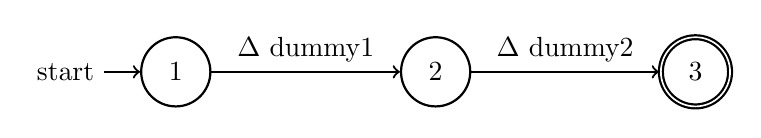
\begin{tikzpicture}[node distance={33mm}, thick, main/.style = {draw,circle}] 
          \node[initial, state] (n_1) {1};
          \node[state] (n_2) [right of=n_1] {2};
          \node[state,accepting] (n_3) [right of=n_2] {3};
          
          \draw[->] (n_1) -- node[midway, above, pos=0.5] {$\Delta$ dummy1} (n_2);
          \draw[->] (n_2) -- node[midway, above, pos=0.5] {$\Delta$ dummy2} (n_3);
        \end{tikzpicture}
    }
    \caption{Local view of the \texttt{main} actor}
    \label{local:main}
\end{figure}

\begin{figure}[!ht]
    \centering
    \resizebox{.8\textwidth}{!}{%
        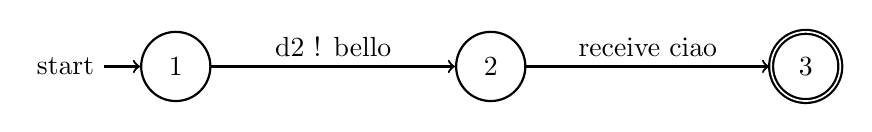
\begin{tikzpicture}[node distance={40mm}, thick, main/.style = {draw,circle}] 
          \node[initial, state] (n_1) {1};
          \node[state] (n_2) [right of=n_1] {2};
          \node[state, accepting] (n_3) [right of=n_2] {3};
          
          \draw[->] (n_1) -- node[midway, above, pos=0.5] {d2 ! bello} (n_2);
          \draw[->] (n_2) -- node[midway, above, pos=0.5] {receive ciao} (n_3);
        \end{tikzpicture}
    }
    \caption{Local view of the \texttt{dummy1} actor}
    \label{local:dummy1a}
\end{figure}

\begin{figure}[!ht]
    \centering
    \resizebox{.8\textwidth}{!}{%
        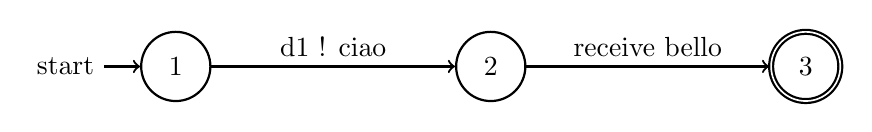
\begin{tikzpicture}[node distance={40mm}, thick, main/.style = {draw,circle}] 
          \node[initial, state] (n_1) {1};
          \node[state] (n_2) [right of=n_1] {2};
          \node[state, accepting] (n_3) [right of=n_2] {3};
          
          \draw[->] (n_1) -- node[midway, above, pos=0.5] {d1 ! ciao} (n_2);
          \draw[->] (n_2) -- node[midway, above, pos=0.5] {receive bello} (n_3);
        \end{tikzpicture}
    }
    \caption{Local view of the \texttt{dummy2} actor}
    \label{local:dummy2a}
\end{figure}

After associating the local views with the actors, the algorithm generates 
the global view shown in Figure \ref{global:async}. 
The automaton expresses two possible global 
executions of the program: from State 1 to State 3, the actors \texttt{dummy1} 
and \texttt{dummy2} are spawned. Then, since the \textit{send} operation is 
non-blocking, either \texttt{dummy1} sends \texttt{ciao} first (leading to 
State 6) or \texttt{dummy2} sends \texttt{bello} first (leading to State 4). 
Consequently, the final state is reached through two possible paths, 
depending on the order in which messages are received.

\begin{figure}[!ht]
    \centering
    \resizebox{\textwidth}{!}{%
        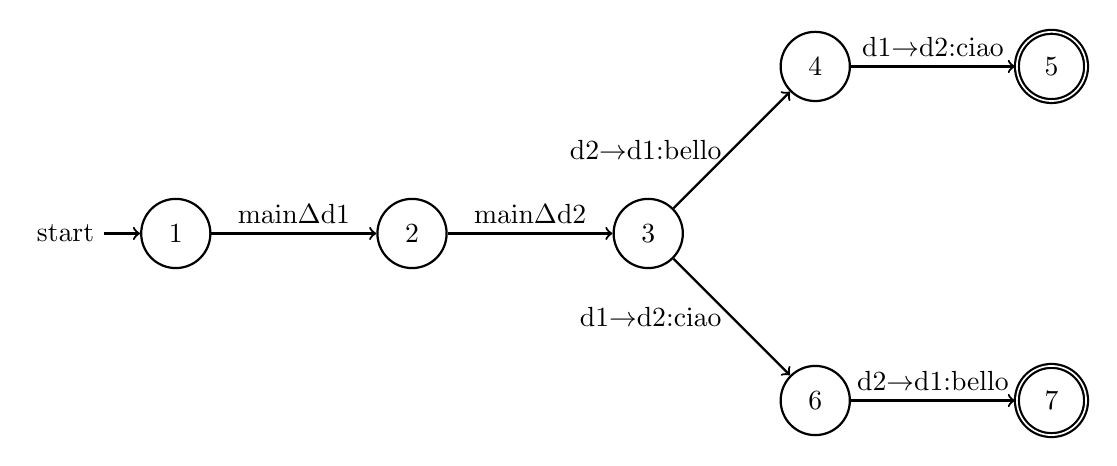
\begin{tikzpicture}[node distance={30mm},thick,main/.style={draw,circle}] 
          \node[initial, state] (n_1) {1};
          \node[state] (n_2) [right of=n_1] {2};
          \node[state] (n_3) [right of=n_2] {3};
          \node[state] (n_4) [above right of=n_3] {4};
          \node[state,accepting] (n_5) [right of=n_4] {5};
          \node[state] (n_6) [below right of=n_3] {6};
          \node[state,accepting] (n_7) [right of=n_6] {7};
          
          \draw[->] (n_1) -- node[midway, above, pos=0.5] {main$\Delta$d1} (n_2);
          \draw[->] (n_2) -- node[midway, above, pos=0.5] {main$\Delta$d2} (n_3);
          \draw[->] (n_3) -- node[midway, left, pos=0.5] {d2$\to$d1:bello} (n_4);
          \draw[->] (n_4) -- node[midway, above, pos=0.5] {d1$\to$d2:ciao} (n_5);
          \draw[->] (n_3) -- node[midway, left, pos=0.5] {d1$\to$d2:ciao} (n_6);
          \draw[->] (n_6) -- node[midway, above, pos=0.5] {d2$\to$d1:bello} (n_7);
        \end{tikzpicture}
    }
    \caption{Global view of Listing \ref{code:async}}
    \label{global:async}
\end{figure}
\end{exmp}

% inserire in appendice le definizioni, la grammatica, algoritmi
% link all'appendice per le versioni formali
% esempi che fanno vedere le differenze tra il prima e il dopo

\subsection{Description of the tool}

\paragraph{How to use the tool}
The tool can be used from the command line interface (CLI). It can be used by compiling each module from the Erlang Shell (Eshell) or, more conveniently, by using \texttt{rebar3}, a standard build tool that provides various features such as package management for community-created libraries, compilation, and automated project testing. By cloning the project from the public GitHub repository and running the \texttt{rebar3 escriptize} command in the main directory, \texttt{rebar3} will, in this order, check for and download dependencies if needed, compile the project, and run tests if present. After that, an executable can be used in \texttt{./\_build/default/bin/chorer}.

\begin{lstlisting}[caption=Usage message]
Usage:
  chorer <input> <entrypoint> <output> <ming> <gstate> <minl>

Extract a choreography automata of an Erlang program.

Arguments:
  input      Erlang soure file (string)
  entrypoint Entrypoint of the program (atom)
  output     Output directory for the generated dot files (string), default: ./
  ming       Minimize the globalviews , default: false
  gstate     Global state are formed with previous messages , default: true
  minl       Minimize the localviews , default: true
\end{lstlisting}

\noindent The mandatory arguments are:
\begin{itemize}
    \item \textbf{Input}: The relative path string of the input Erlang program, from which the tool will generate local and global views.
    \item \textbf{Entrypoint}: The atom representing the function where the execution of the input program begins. This parameter is essential because Erlang does not have a conventional entry point function (i.e. the main in C, but in Erlang can be every exported function). It will be passed to the function that creates the global view to start the simulation.
\end{itemize}

\noindent The optional arguments are:
\begin{itemize}
    \item \textbf{Output}: The relative path string of the output folder where the local and global view files will be saved. Local views will be named \texttt{[function name with arity]\_local\_view.dot}, while the global view file will be named \texttt{[Entrypoint]\_global\_view.dot}.
    \item \textbf{Options}: Currently, this is a tuple of two booleans that allow customization of local views. The first boolean determines whether to identify final states (by default, it is set to true). The second adds more information to the local view by including transitions related to other language constructs in addition to communication constructs (by default, it is set to false). This parameter may be expanded in the future with additional booleans.
\end{itemize}

\begin{lstlisting}[language=Erlang, caption=Use example of the tool]
 shell> ./_build/default/bin/chorer ./path/to/file.erl entrypoint/0
\end{lstlisting}

\paragraph{Struttura del tool}
Il progetto si divide in due cartelle principali. Sotto la cartella \texttt{examples} ci sono vari esempi di programmi in Erlang su cui provare il tool. Il codice del tool si trova invece nella cartella \texttt{src}. 

\bigskip

\dirtree{%
.1 chorer.
.2 examples.
.3 ....
.2 src.
.3 choreography.
.4 actor\_emul.erl.
.4 eval.erl.
.4 gv.erl.
.4 lv.erl.
.4 md.erl.
.3 common.
.4 common\_data.hrl.
.4 db.erl.
.4 digraph\_to\_dot.erl.
.4 fsa.erl.
.4 log.erl.
.4 settings.erl.
.4 share.erl.
.3 chorer\_app.erl.
.3 chorer.app.src.
.2 rebar.config.
.2 rebar.lock.
}

\bigskip

Il file principale \`e \texttt{chorer\_app.erl}, dove si trova la funzione \texttt{start}. I file \texttt{rebar.config}, \texttt{rebar.lock} e \texttt{chorer.app.src} servono a far funzionare il tool \texttt{rebar3}. Nella cartella \texttt{choreography} si trovano i moduli adibiti all'analisi statica del programma e alla creazione delle viste locali e globali. In particolare, il modulo \texttt{db\_manager.erl} si occupa della gestione di dati in comune, utile per non passare tanti dati attraverso i parametri delle funzioni. I moduli \texttt{metadata.erl}, \texttt{local\_view.erl} e \texttt{global\_view.erl} si occupano rispettivamente di gestire l'estrazione dei dati preliminari, la creazione delle viste locali e la creazione della vista globale. Invece, nella cartella \texttt{common} si trovano le funzioni ``in comune" per tutti i moduli, quindi la gestione e minimizzazione degli automi (in \texttt{fsa.erl}), la conversione di un grafo in formato DOT (in \texttt{digraph\_to\_dot.erl}) e il salvataggio su file (in \texttt{common\_fun.erl}). Il file \texttt{common\_data.hrl} contiene le strutture dati utilizzate nel progetto.


\subsubsection{From Erlang to Choreographies}
\label{sec:corrisp}
In questa sezione, verranno definite le corrispondenze tra codice in Erlang e automa coreografico, rispettivamente per viste locali e globali.

\paragraph{Viste locali}

Il codice di un'operazione \texttt{receive} (come nel codice \ref{code:receive}) corrisponde al grafo \ref{grafo:receive}; ogni ramo verr\`a valutato ricorsivamente, continuando quindi la costruzione dai rami; infine, tutti i rami si ricongiungeranno su un nodo comune con delle transizioni $\epsilon$, dal quale ripartir\`a la valutazione della vista locale. L'operazione \texttt{Pid ! message} corrisponde al grafo \ref{grafo:send}. La chiamata alla funzione \texttt{spawn} corrisponde al grafo \ref{grafo:spawn}.

\bigskip

\begin{figure}[ht!]
    \centering
    \begin{tikzpicture}[node distance={29mm}, thick, main/.style = {draw, circle}] 
      \node[state] (n_1) {1};
      \node[state] (n_2) [above right of=n_1] {2};
      \node[state] (n_4) [below right of=n_1] {$n$};
      \node[state] (n_3) [below=\distance cm of n_2] {\ldots};
      \node[state] (n_5) [right of=n_2] {\ldots};
      \node[state] (n_6) [right of=n_3] {\ldots};
      \node[state] (n_7) [right of=n_4] {$m$};
      \node[state] (n_8) [below right of=n_5] {$m+1$};
      
      \draw[->] (n_1) -- node[midway, above left, pos=0.6] {receive message1} (n_2);
      \draw[->] (n_1) -- node[midway, above, pos=0.5] {...} (n_3);
      \draw[->] (n_1) -- node[midway, below left, pos=0.6] {receive messageN} (n_4);
      \draw[->] (n_2) -- node[midway, above, pos=0.5] {...} (n_5);
      \draw[->] (n_3) -- node[midway, above, pos=0.5] {...} (n_6);
      \draw[->] (n_4) -- node[midway, above, pos=0.5] {...} (n_7);
      \draw[->] (n_5) -- node[midway, above, pos=0.5] {$\epsilon$} (n_8);
      \draw[->] (n_6) -- node[midway, above, pos=0.5] {$\epsilon$} (n_8);
      \draw[->] (n_7) -- node[midway, above, pos=0.5] {$\epsilon$} (n_8);
    \end{tikzpicture}
    \caption{Grafo locale per il costrutto \texttt{receive}}
    \label{grafo:receive}
\end{figure}


\begin{figure}[ht!]
    \centering
    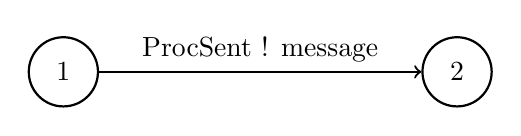
\begin{tikzpicture}[node distance={50mm}, thick, main/.style = {draw, circle}] 
      \node[state] (n_1) {1};
      \node[state] (n_2) [right of=n_1] {2};
      
      \draw[->] (n_1) -- node[midway, above, pos=0.5] {ProcSent ! message} (n_2);
    \end{tikzpicture}
    \caption{Grafo locale per il costrutto \texttt{!}}
    \label{grafo:send}
\end{figure}

\bigskip

\begin{figure}[ht!]
    \centering
    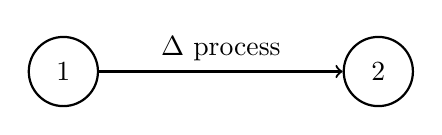
\begin{tikzpicture}[node distance={40mm}, thick, main/.style = {draw, circle}] 
      \node[state] (n_1) {1};
      \node[state] (n_2) [right of=n_1] {2};
      
      \draw[->] (n_1) -- node[midway, above, pos=0.5] {$\Delta$ process} (n_2);
    \end{tikzpicture}
    \caption{Grafo locale per il costrutto \texttt{spawn}}
    \label{grafo:spawn}
\end{figure}


\paragraph{Chiamate di funzioni}
Essendo un linguaggio di programmazione funzionale, vengono eseguite numerose chiamate di funzione. Le funzioni possono essere presenti nello stesso file, in un modulo differente, oppure possono essere funzioni \textit{built-in}. Di seguito vengono mostrate le chiamate di funzioni che modificano il comportamento del grafo.

\paragraph{Chiamate ricorsive}

Nel caso delle chiamate \textit{ricorsive}, si crea una transizione $\epsilon$ dall'ultimo nodo creato fino al primo nodo, come mostrato in figura \ref{grafo:ricors}.

\begin{figure}[ht!]
    \centering
    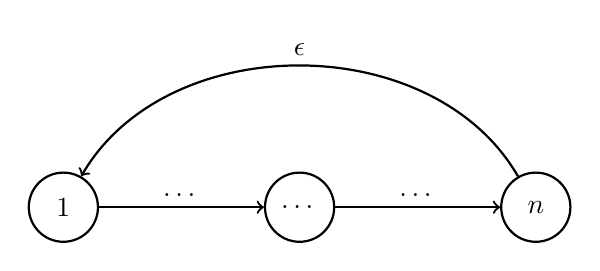
\begin{tikzpicture}[node distance={3cm}, thick, main/.style = {draw, circle}] 
      \node[state] (n_1) {1};
      \node[state] (n_2) [right of=n_1] {\ldots};
      \node[state] (n_3) [right of=n_2] {$n$};
      
      \draw[->] (n_1) -- node[midway, above, pos=0.5] {\ldots} (n_2);
      \draw[->] (n_2) -- node[midway, above, pos=0.5] {\ldots} (n_3);
      \draw[->] (n_3) to [out=120,in=60] node[midway, above, pos=0.5] {$\epsilon$} (n_1);
    \end{tikzpicture}
    \caption{Grafo della chiamata ricorsiva di una funzione}
    \label{grafo:ricors}
\end{figure}

\paragraph{Chiamata a una funzione generica}
Quando si incontra in chiamata ad una funzione non conosciuta, l'algoritmo creer\`a la vista locale della funzione chiamata e ``collegher\`a" l'inizio del grafo della funzione chiamata con l'ultimo stato creato nella vista locale della funzione chiamante, collegandolo con una transizione $\epsilon$. La vista locale continuer\`a dall'ultimo vertice del grafo della chiamata.

\bigskip

\begin{figure}[ht!]
    \centering
    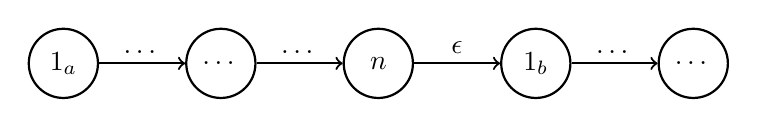
\begin{tikzpicture}[node distance={2cm}, thick, main/.style = {draw, circle}] 
      \node[state] (n_1) {$1_a$};
      \node[state] (n_2) [right of=n_1] {\ldots};
      \node[state] (n_3) [right of=n_2] {$n$};
      \node[state] (n_4) [right of=n_3] {$1_b$};
      \node[state] (n_5) [right of=n_4] {\ldots};
      
      \draw[->] (n_1) -- node[midway, above, pos=0.5] {\ldots} (n_2);
      \draw[->] (n_2) -- node[midway, above, pos=0.5] {\ldots} (n_3);
      \draw[->] (n_3) -- node[midway, above, pos=0.5] {$\epsilon$} (n_4);
      \draw[->] (n_4) -- node[midway, above, pos=0.5] {\ldots} (n_5);
    \end{tikzpicture}
    \caption{Grafo di una chiamata di funzione}
    \label{grafo:funcall}
\end{figure}

Nel grafo \ref{grafo:funcall}, lo stato $1_a$ \`e lo stato iniziale della funzione chiamante e lo stato $1_b$ indica il primo stato della vista locale della funzione chiamata.

\paragraph{Viste globali}

Per le viste globali, nelle \texttt{spawn} si specifica l'attore che esegue l'operazione a sinistra del simbolo come mostrato nella figura \ref{grafo:globspawn}. Una spawn verr\`a direttamente inserita nel grafo. Ogni processo verr\`a anche numerato, nel caso vengano creati molteplici attori per la stessa funzione.

\bigskip

\begin{figure}[ht!]
    \centering
    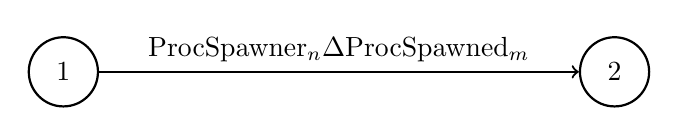
\begin{tikzpicture}[node distance={7cm}, thick, main/.style = {draw, circle}] 
      \node[state] (n_1) {1};
      \node[state] (n_2) [right of=n_1] {2};
      
      \draw[->] (n_1) -- node[midway, above, pos=0.5] {ProcSpawner$_n\Delta$ProcSpawned$_m$} (n_2);
    \end{tikzpicture}
    \caption{Grafo globale per il costrutto \texttt{spawn}}
    \label{grafo:globspawn}
\end{figure}

\bigskip

Per l'invio e la ricezione di messaggi, durante la simulazione degli attori, se vengono trovati due attori che eseguono una send e una receive compatibile, allora verr\`a aggiunta alla vista globale uno stato come in figura \ref{grafo:sendrecv}. Per essere compatibili, il processo ricevente deve corrispondere al destinatario dei dati e il pattern matching della receive deve combaciare con i dati inviati. Le transizioni \textit{send} e \textit{receive} fatte a ``vuoto" (cio\`e i messaggi che vengono inviati, ma non vengono processati da una \textit{receive} di un qualsiasi processo) non verranno mostrate nell'automa globale.

\bigskip

\begin{figure}[ht!]
    \centering
    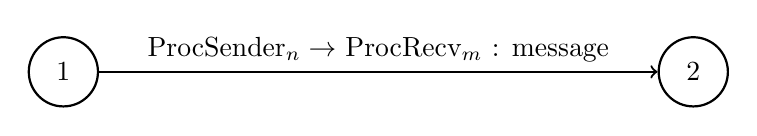
\begin{tikzpicture}[node distance={8cm}, thick, main/.style = {draw, circle}] 
      \node[state] (n_1) {1};
      \node[state] (n_2) [right of=n_1] {2};
      
      \draw[->] (n_1) -- node[midway, above, pos=0.5] {ProcSender$_n\to$ ProcRecv$_m$ : message} (n_2);
    \end{tikzpicture}
    \caption{Grafo globale per \texttt{receive} e \texttt{!}}
    \label{grafo:sendrecv}
\end{figure}


\subsubsection{Main algorithms}
Execution is divided into 3 main phases:
\begin{enumerate}
    \item Initialization of the \texttt{db\_manager}, data structures, and extraction of preliminary information (handled by the \texttt{metadata.erl} module): possible actors are extracted from the \texttt{export} attribute, the number of \texttt{spawn} executions is counted, and the ASTs of all functions are saved in the \texttt{db\_manager}. Meanwhile, an initial evaluation of the program flow is performed by initializing the names of actors and saving the argument passing to the \texttt{spawn} functions.
    \item Creation of local views for all possible actors, i.e., all functions that appear in the \texttt{export} at the beginning of a program (obtained from the first phase).
    \item Creation of the global view starting from the program's starting point and combining the local views created in phase two.
\end{enumerate}


\paragraph{Module \texttt{local\_view.erl}}
In the module that creates local views, the main function is \texttt{eval\_codeline}. This function evaluates the individual line of code and its arguments. It also adds nodes to the local view graph in the case of communication constructs. The function creates a binding between a variable and its content, if evaluable. Additionally, it creates branches with $\epsilon$ edges in the case of \texttt{if} and \texttt{case}. Later, the $\epsilon$ transitions will be eliminated through graph minimization. There are also some evaluations of useful \textit{built-in} functions for communication, such as \texttt{self()} which returns the ID of its own process and \texttt{register} which registers a process ID in an \textit{atom}.
Below is the pseudocode of some interesting branches.

\begin{lstlisting}[language=Erlang, caption=Pseudocode of \texttt{eval\_codeline} function, label=code:eval]
eval_codeline(CodeLine, FunctionName, UsefulData) ->
    case CodeLine of
        %%% Eval recursive call
        {call, _, {atom, _, FunctionName}, ArgList} ->
            manage_recursive_call();
        %%% Evaluate the spawn function
        {call, _, {atom, _, spawn}, ArgList} ->
            add_spawn_to_local_view();
        %%% Evaluate a call to a generic function
        {call, _, {atom, _, Name}, ArgList} ->
            manage_call();
        %%% Eval Var = something
        {match, _, RightContent, LeftContent} ->
            manage_var();
        %%% Evaluate case with pattern matching
        {'case', _, Data, PMList} ->
            manage_case();
        %%% Evaluate if like case
        {'if', _, PMList} ->
            manage_if();
        %%% Evaluate receive with pattern matching
        {'receive', _, PMList} ->
            add_receive_to_local_view();
        %%% Evaluate send
        {op, _, '!', ProcSent, DataSentAst} ->
            add_send_to_local_view();
        %%% Evaluate data types
        {atom, _, Value} -> return_var();
        {integer, _, Value} -> return_var();
        {string, _, Value} -> return_var();
        ...
        _ -> nomatch
    end.
\end{lstlisting}

\textbf{N.B.}: In Erlang, it is rare to specify from which process you want to receive a particular message because it is not known in advance which actors are present. Therefore, the global view will use the label \texttt{receive msg} to express the branch where a specific message is received. Pattern matching will also be specified, evaluating where possible, to facilitate the creation of the global view.

In section \ref{sec:corrisp}, the correspondence between code and graph for constructs that modify the local view will be explicitly stated. Instead, the branches corresponding to data types or \textit{built-in} functions (like \texttt{self()}) return a data structure representing the data, which will either be bound to a variable in the \texttt{match} branch or passed as an argument to a function.

\paragraph{Module \texttt{global\_view.erl}}

While creating a local view simply involves following the function code line by line, in the global view, we need to compose the local views while taking into account the various actors created. Therefore, an approximate execution will be simulated starting from the startup function. Each actor will be associated with a process of the \texttt{proc\_loop} function, which keeps track of available branches and the state of the process. This function is responsible for providing the main process with some information related to the actor.

\begin{lstlisting}[language=Erlang, caption=Pseudocode of \texttt{proc\_loop} function]
proc_loop(LocalView, CurrentState, MarkedEdges) ->
    receive
        {use_transition, Edge} ->
            % to avoid infinite loops
            NewState = verify_not_marked();
            proc_loop(LocalView, NewState, MarkedEdges);
        {P, get_info} ->
            P ! {someinfo},
            proc_loop(LocalView, CurrentState, MarkedEdges);
        stop -> terminated
    end.
\end{lstlisting}

Furthermore, messages could travel either within the same virtual machine or across the network, so message exchange occurs asynchronously. That is, if two sends, $A$ and $B$, are made to the same process, either $A$ or $B$ could arrive first, completely changing the execution flow of the program.

In the following code \ref{code:global}, the main function of the \texttt{global\_view.erl} module is presented, which creates the global view by combining actors and their local views. The basic idea is to create a \textit{depth-first view} (DFS) of the actor automata, stopping appropriately according to the communication rules.

\begin{lstlisting}[language=Erlang, caption=Main function for globalview construction, label=code:global]
progress_branches(BranchList) ->
    NewBranchList = lists:foreach(
        fun(Item) -> progress_single_branch(Item) end,
        BranchList
    ),
    progress_branches(NewBranchList).
progress_single_branch(Data) ->
    SendList = lists:foreach(
        fun(Name) -> eval_proc_until_send(Name) end,
        Data.proc_list
    ),
    lists:foreach(
        fun(SendData) -> 
            manage_send(duplicate_branch(SendData))
        end,
        SendList
    ).
\end{lstlisting}

The strategy for composing local views is to have all actors continue until any \textit{send} (line 3 of code \ref{code:global}). While searching for and finding the first \textit{send}, \textit{spawn} and \textit{receive} are also searched. If a \textit{spawn} is encountered, the corresponding node is immediately added to the graph, and the actor is created. If a \textit{receive} is encountered, the message queue of the process is checked. If a compatible message is found, a transition is created on the graph, and the two actors continue execution.

After being blocked on a \textit{send} or \textit{receive}, processes will be duplicated on different branches for different executions (line 14 of code \ref{code:global}). Each "branch" of execution will differ depending on which \textit{send} is evaluated first. At the same time, a check is performed to see if a process is available to receive that message. If so, a transition is created on the global graph, and the actors continue. Otherwise, the "vacant" \textit{send} is inserted into an appropriate data structure.

The algorithm in \ref{code:global} is executed recursively until a relevant data structure is modified (such as the graph). On the first iteration that does not modify any data structure, the algorithm stops. The final graph will represent the communication that occurred asynchronously for messages sent from different actors. Examples of "branching" between \textit{send}s are shown in the example section.

Each module, after creating their respective automata, will be responsible for converting them into DOT language and saving them to a file. To visualize the graphs, simply copy the contents of the file into an application that interprets the DOT format.


\paragraph{Old state}

The tool can accurately parse the main constructs and features of the Erlang language. In Table \ref{erl}, we outline the current status: what is supported, what is not supported, and what are the next objectives. It was decided not to support certain constructs because they are not useful at this stage of the project. For example, supporting error handling with try-catch is unnecessary when variable passing is not yet implemented. Additionally, some constructs were excluded because they are orthogonal to others, such as complex data structures. The tool generates a local view that closely aligns with the behavior of the original actor, and the algorithm for combining local views into a global view performs well on simple examples. However, at present, it does not provide automatic error detection for certain properties in the global choreography.

% \begin{table}[!ht]
%     \centering
%     \begin{minipage}{0.49\textwidth}
%     \centering
%     \begin{tabular}{|c||c|}
%     \hline \textbf{Keyword} & \textbf{Support}    \\  \hline
%      atom & \cellcolor{ashgrey}yes    \\  \hline
%      integer & \cellcolor{ashgrey}yes \\   \hline
%      float &\cellcolor{ashgrey}yes    \\   \hline
%      boolean &\cellcolor{ashgrey}yes    \\   \hline
%      tuple & \cellcolor{ashgrey}yes    \\   \hline
%      list &\cellcolor{ashgrey}yes    \\   \hline
%      record & \cellcolor{red!50}no   \\   \hline
%      map & \cellcolor{red!50}no   \\   \hline
%      binary & \cellcolor{red!50}no    \\   \hline
%      if & \cellcolor{ashgrey}yes    \\   \hline
%      case & \cellcolor{ashgrey}yes    \\   \hline
%      receive &\cellcolor{ashgrey}yes    \\   \hline
%     \end{tabular}
%     \end{minipage}
%     \centering
%     \begin{minipage}{0.49\textwidth}
%     \begin{tabular}{|c||c|}
%     \hline \textbf{Keyword} & \textbf{Support}    \\  \hline
%      ! & \cellcolor{ashgrey}yes    \\   \hline
%      assignment &\cellcolor{ashgrey}yes    \\   \hline
%      function & \cellcolor{green!50}goal  \\   \hline
%      recursion & \cellcolor{green!50}goal   \\   \hline
%      hof &\cellcolor{green!50}goal    \\   \hline
%      when & \cellcolor{red!50}no    \\   \hline
%      self &\cellcolor{ashgrey}yes    \\   \hline
%      spawn &\cellcolor{ashgrey}yes    \\   \hline
%      rand:uniform &\cellcolor{ashgrey}yes    \\   \hline
%      try catch & \cellcolor{red!50}no    \\   \hline
%      after & \cellcolor{red!50}no    \\   \hline
%      math operation &\cellcolor{red!50}no    \\   \hline
%     \end{tabular} 
%     \end{minipage}
    
%     \caption{Supported constructs: Keywords in gray are already supported, keywords in red are not supported and are unlikely to be supported soon. Constructs in green are related to functions, because parameter passing is not supported.}
%     \label{erl}
% \end{table}

\section{Contributions}
\subsection{Attributed grammar}
To better understand how the parsing of a file and the creation of a localview 
should work, we created an attributed grammar for a subset of the Erlang language.
An attributed grammar extends a context-free grammar by associating attributes with 
its symbols and defining semantic rules. Attributes can be \textit{synthesized} (computed 
from child nodes) or \textit{inherited} (passed from parent nodes). These rules define how 
information propagates through the parse tree. In the following attributed grammar, 
we define the localview of Chorer's constructs.

\paragraph{Program}

$prog \to (funPattern)^+$

A program doesn't have a local-view, no need to write attributes.

\paragraph{Function 
}
\paragraph{List}

$funList \to (funPattern)^+$

We create only the local-views that we need.

\paragraph{Pattern}

Base case: $funPattern \to fun.$ (trivial)

$funPattern \to fun_1;...;fun_N.$

\begin{verbatim}
funPattern.nodes = new U fun1.nodes U ... U funN.nodes
funPattern.edges = link(new,fun1.first) U ... U 
                   link(new,funN.first) U 
                   fun1.edges U ... U funN.edges
funPattern.first = new
\end{verbatim}

\paragraph{Body}

$fun \to Atom(X_1,...,X_n) \to Exprs$

Attributes:
\begin{verbatim}
fun.nodes = new U Exprs.nodes
fun.edges = Exprs.edges U link(new, E.first)
fun.first = new
fun.last = Exprs.last
fun.context = [ X1 -> Param[1], ..., Xn -> Param[n] ]
fun.ret_var = E.ret_var
\end{verbatim}

\texttt{Param} is taken as input (default to \texttt{ANYDATA})

\paragraph{Expressions}

\paragraph{Concatenation}

Base case: $Exprs \to expr$ (trivial)

$Exprs \to expr,Exprs'$

Attributes:
\begin{verbatim}
Exprs.nodes = expr.nodes U Exprs'.nodes
Exprs.edges = expr.edges 
              U Exprs'.edges 
              U link(expr.last, Exprs'.first, epsilon)
Exprs.first = expr.first
Exprs.last = Exprs'.last
Exprs.context = expr.context U Exprs'.context
Exprs.ret_var = Exprs'.ret_var
\end{verbatim}

\paragraph{Send}

$expr \to expr'\ \ !\ \ expr''$

Attributes:
\begin{verbatim}
expr.nodes = expr'.nodes U expr''.nodes U new1 U new2
expr.edges = expr'.edges U expr''.edges
             U link(expr''.last, new1, epsilon)
             U link(new1, new2, expr'.ret_var 
                + " ! " 
                + expr''.ret_var)
expr.first = expr'.first
expr.last = new2
expr.context = expr'.context U expr''.context
expr.ret_var = expr''.ret_var
\end{verbatim}

Firstly evaluate the left-hand side expression, then the right hand side one. 
Lastly insert the sends edge.

\paragraph{Receive}

$expr \to receive patter_1 \to Exprs_1; ...; pattern_n \to Exprs_n end$

Attributes:
\begin{verbatim}
expr.first = new1
expr.last = new2
expr.nodes = Exprs1.nodes U ... U Exprsn.nodes U new1 U new2
expr.edges = Exprs1.edges U ... U Exprsn.edges
             U link(new1, Exprs1.first, epsilon) 
             U ...
             U link(new1, Exprsn.first, epsilon)
             U link(Exprs1.last, new2, epsilon)
             U ...
             U link(Exprsn.last, new2, espilon)
expr.ret_var = ANYDATA (overapprox)
context?
\end{verbatim}

\paragraph{Spawn call}

$expr \to spawn(Atom, Params)$

Attributes:
\begin{verbatim}
expr.nodes = new1 U new2
expr.edges = link(new1, new2, "spawn Atom")
expr.first = new1
expr.last = new2
expr.ret_var = newVar(type: pid, value: random) 
\end{verbatim}

\paragraph{Recursive call}

$expr \to FunName(Params)$

Attributes:
\begin{verbatim}
expr.edges = expr.edges U link(FunName.first, expr.last)
expr.ret_var = null
\end{verbatim}

Use of inherited attributes
Stop evaluation

\paragraph{Generic function call} 

$expr \to Atom(Params)$

Attributes:
\begin{verbatim}
G = get_localview(Atom, Param)
expr.nodes = G.nodes
expr.edges = G.edges
expr.first = G.first
expr.last = G.last
expr.ret_var = G.ret_var 
\end{verbatim}

\paragraph{Assignment}

$expr \to pattern = expr'$

Attributes:
\begin{verbatim}
expr.nodes = expr'.nodes
expr.edges = expr'.edges
expr.first = expr'.first
expr.last = expr'.last
expr.context = [pattern -> expr'.ret_var]
\end{verbatim}

\subsection{Improvements on the tool}
One key goal of the tool is to generate correct graph outputs, ensuring an  
accurate representation of program behavior. While refining abstract aspects  
of the project, several features, improvements, and bug fixes have been added  
to enhance the precision and consistency of the global view specification. The  
iterative process of refining the tool aims to minimize errors, and provide a
more reliable emulation of  actor-based execution. Future work will continue to
focus on refining these aspects to offer greater 
flexibility while maintaining correctness of the analyzed program.

\paragraph{Features}
Two key features have been added to the tool. The first one improves the local  
view module. The tool can now correctly parse programs where values are passed   
as arguments to functions, allowing for a more precise representation of  
data flow between processes. 
Previously, only functions without value passing were supported. This was a
significant limitation and, in fact, one of the highest-priority features.
It was the final major feature of a programming language to be added, and it is 
now included in the parsing module, enabling a broader range of program inputs.

The second feature added to the tool enhances over-approximation
in the global view module. During computation, the value of 
some data can become everything because we cannot know the outcome of an 
operation performed on the data (i.e. we don't support mathematical operation). 
The tool now substitutes this unknown value with the \texttt{ANY} keyword to 
indicate that it can represent any kind of data. If a message is exchanged with 
\texttt{ANY} as its content, it will match every possible receive branch,
ensuring a more over-approximated analysis of the program.

\paragraph{General improvements}
Some general improvements have been made on the tool. 
The tool is now more resilient to unexpected errors, reducing the  
likelihood of crashes and ensuring that it provides meaningful output in  
most cases, even when encountering invalid input. This was achieved through the
implementation of more error checks and recovery patterns within the codebase, 
where there were none before.

Also, a new library has been integrated for command-line argument management,  
making the CLI more robust and user-friendly, with better parsing of  
parameters and improved error messages.

Some effort has been put to improve the testing environment and benchmark 
generation. The tool now produces useful benchmarking information, which is 
processed by a dedicated Python script. This script collects and analyzes the 
data to generate meaningful performance benchmarks. Additionally, if the  
\texttt{correct\_gv.dot} file is present (that is a dot file containing 
the expected global view) the script performs an automatic correctness check. 
This feature lays the groundwork for more expressive and rigorous testing in 
the future, enabling better validation of the tool's accuracy and performance
across different scenarios and use cases.

\paragraph{Bug fixes}
Some notable bug fix improvements were made within the global view module that 
are needed to be mentioned. It has been resolved an issue where the tool
incorrectly printed warnings about failing to find the correct process during
the sending of a message. This bug caused the useless show of some false 
positive warnings. 

It also has been addressed a problem that prevented the exploration of certain
branches during the global view emulation, ensuring a more comprehensive
traversal of all possible execution paths. This bug prevented a full branch
exploration in certain programs. 

It has been fixed a bug that was causing excessive duplicate branches. 
This patch corrected an issue where unnecessary duplicate branches were created  
after receiving a message and defining a new variable. This fix improves  
the accuracy of the global view by reducing redundant computations.  


\subsection{Benchmarks}
Significant effort has been dedicated to developing a 
generic and automated script (written in Python) to test the tool and extract 
relevant information about the tool and its output.
Table~\ref{tab:gvbench} presents empirical data on the evaluation of various 
examples processed by the tool. 
The examples are primarily designed ad hoc to test specific aspects of the tool.
They are not sourced from well-known Erlang suites, as the tool is still in an
early stage and cannot yet parse most of them.
The columns of Table~\ref{tab:gvbench} provide the following information:

\begin{itemize}
    \item \textbf{Example}: Name of the test case.
    \item \textbf{Lines}: Number of lines of code in the example.
    \item \textbf{Tot LV}: Total number of local views generated by the example.
    \item \textbf{GV Nodes}: Number of nodes in the global view graph.
    \item \textbf{GV Edges}: Number of edges in the global view graph.
    \item \textbf{Warns}: Number of warnings raised.
    \item \textbf{Errors}: Number of errors detected (i.e. deadlocks).
    \item \textbf{Time}: Execution time in seconds.
\end{itemize}

The entries are ordered by the number of lines of code. The generated graphs 
included in the table are presented without minimization. Applying minimization 
techniques to the global view graph can lead to incorrect reductions in some 
cases, cause of a known bug. Therefore, we opted to maintain the full 
graph representation to ensure correctness.

\paragraph{Analysis of global view empirical data}
From the Table~\ref{tab:gvbench}, we can observe the overall behavior of the tool, 
focusing on the number of warnings and errors in the output. 
As previously mentioned, a high number of message exchanges directly correlates  
with an increased number of nodes and edges in the global view.
Warnings usually occur when the
tool encounters unknown elements in the source code, such as a new keyword or
an external function. They also appear when the tool loses track of a process
identifier, preventing it from mapping message exchanges correctly. 
This occurs in the \texttt{if-cases} example, which generates 185 warnings due to
the tool's failure to instantiate a variable with the correct process identifier,
making it unable to deliver the corresponding message. This issue likely stems 
from a bug in the actor emulation module.
Errors typically arise when an unexpected situation occurs or when a deadlock
state is detected. Most examples do not automatically terminate a process once
it completes its task (e.g., waiting for requests), which contributes to this
issue. However, one particularly notable case is \texttt{foo8}, which has 561
nodes, 560 edges, and 191 errors. The reason lies in its heavy use of case
constructs—some information is lost between the local and global views, leading
the tool to explore every possible execution path. This results in a high number
of states, edges, and undefined deadlock conditions. 
Using a minimized version of the local graph during actor emulation can
significantly reduce these values. However, this conflicts with the principle
of using an over-approximated approach. To address this, minimization could be
added as a program argument, allowing users to trade some generality for a
more precise global view graph.

\paragraph{About complexity}
A significant portion of the execution time is obviously consumed by the global  
view composition algorithm. This algorithm attempts to explore all possible  
program executions, considering every potential message order to meet the  
overapproximation requirement. In the worst-case scenario, without any  
restrictions, it must evaluate all permutations of messages, resulting in a  
factorial time complexity of \( O(n!) \). However, in most cases, more efficient  
strategies can be applied to mitigate this complexity.
The execution times show that our algorithm performs efficiently even on large 
examples (an example is considered large when there are many nodes and edges
because this corresponds to a high number of messages exchanged, leading to a
high number of possible combination of these messages), with the most complex 
cases (e.g., \texttt{foo8}) taking only a few seconds.

\begin{table}[!ht]
\centering
\begin{tabular}{|c|c|c|c|c|c|c|c|}
\hline
Example & Lines & Tot LV & GV Nodes & GV Edges & Warns & Errors & Time \\ 
\hline
unknown & 13 & 2 & 2 & 2 & 0 & 0 & 0.175s \\ 
foo9 & 14 & 4 & 4 & 3 & 1 & 3 & 0.187s \\ 
foo9c & 15 & 3 & 10 & 15 & 0 & 0 & 0.182s \\ 
pass & 16 & 3 & 3 & 2 & 0 & 0 & 0.174s \\ 
foo9d & 16 & 3 & 3 & 2 & 0 & 0 & 0.186s \\ 
funcall & 17 & 3 & 4 & 3 & 1 & 2 & 0.180s \\ 
forloop & 18 & 3 & 7 & 6 & 0 & 0 & 0.188s \\ 
foo1 & 18 & 3 & 8 & 7 & 0 & 0 & 0.175s \\ 
foo5 & 18 & 3 & 79 & 165 & 1 & 0 & 0.316s \\ 
async & 20 & 3 & 7 & 6 & 0 & 0 & 0.194s \\ 
foo4 & 20 & 4 & 16 & 19 & 0 & 2 & 0.182s \\ 
hof & 21 & 4 & 15 & 17 & 0 & 3 & 0.189s \\ 
foo9b & 21 & 4 & 4 & 4 & 14 & 1 & 0.183s \\ 
spawn & 22 & 3 & 9 & 8 & 0 & 0 & 0.179s \\ 
foo3 & 22 & 3 & 13 & 16 & 0 & 0 & 0.178s \\ 
account & 23 & 3 & 28 & 39 & 0 & 2 & 0.211s \\ 
airline & 23 & 3 & 15 & 26 & 1 & 0 & 0.232s \\ 
foo2 & 23 & 4 & 4 & 3 & 1 & 1 & 0.180s \\ 
foo9h & 23 & 4 & 24 & 35 & 0 & 5 & 0.196s \\ 
hello & 24 & 3 & 5 & 6 & 2 & 0 & 0.190s \\ 
trick & 24 & 4 & 9 & 9 & 0 & 0 & 0.184s \\ 
foo6 & 24 & 5 & 9 & 9 & 15 & 2 & 0.190s \\ 
foo9e & 24 & 5 & 14 & 14 & 0 & 5 & 0.186s \\ 
foo9f & 25 & 5 & 7 & 6 & 0 & 4 & 0.183s \\ 
foo9g & 25 & 5 & 44 & 83 & 0 & 7 & 0.226s \\ 
conditional & 26 & 2 & 25 & 24 & 1 & 16 & 0.197s \\ 
foo8 & 29 & 5 & 561 & 560 & 0 & 191 & 3.590s \\ 
producer & 30 & 4 & 11 & 10 & 0 & 1 & 0.183s \\ 
dining & 31 & 3 & 45 & 72 & 0 & 2 & 0.232s \\ 
ticktackloop & 32 & 4 & 6 & 6 & 2 & 0 & 0.182s \\ 
airline & 33 & 3 & 35 & 68 & 1 & 0 & 0.232s \\ 
ping & 36 & 3 & 6 & 5 & 1 & 0 & 0.188s \\ 
meViolation & 40 & 4 & 63 & 82 & 2 & 4 & 0.266s \\ 
serverclient & 41 & 5 & 9 & 8 & 8 & 3 & 0.187s \\ 
foo7 & 41 & 3 & 149 & 229 & 0 & 6 & 0.513s \\ 
ticktackstop & 46 & 5 & 19 & 27 & 7 & 0 & 0.214s \\ 
purchase & 47 & 5 & 49 & 66 & 6 & 0 & 0.257s \\ 
customer & 54 & 5 & 17 & 22 & 1 & 0 & 0.205s \\ 
if-cases & 57 & 4 & 148 & 210 & 185 & 30 & 0.525s \\ 
\hline
\end{tabular}
\caption{Global view empirical data}
\label{tab:gvbench}
\end{table}

\paragraph{Correctness of Global View}
One of the main contributions was enabling automatic verification of whether a
global view matches its correct version. Since knowing the complete specification
in advance is not trivial, we conducted tests on a few selected examples. 
The correct versions of the graph can be seen as what we expect to be the final
global view.
Table~\ref{tab:corrbench} briefly shows the correctness of the global view. 
The \textbf{Check} column indicates whether the global view 
correctly represents the expected behavior. Some examples, such as 
\texttt{async} and \texttt{ticktackloop}, are correctly generated because they 
are very simple example, while others fail. This may result from a missing 
feature in local or global view generation or from
the expected version not aligning with actual results. A key future goal of the
project is to generate as many correct global view versions as possible and to
systematically check and refine each one.

\begin{table}[!ht]
\centering
\begin{tabular}{|c|c|}
\hline
Example & Check \\ 
\hline
unknown & False \\ 
async & True \\ 
ticktackloop & True \\ 
ticktackstop & False \\ 
customer & False \\ 
\hline
\end{tabular}
\caption{Global view correctness data}
\label{tab:corrbench}
\end{table}



\section{Case studies}
In order to better illustrate the features of the tool, we present in
this section two examples (using Erlang-like, actor-based pseudocode), each one
composed by a pseudocode and the corresponding Choreography
Automata~\cite{coordination2020-chorAuto} of the global view of the
communicating system. Here, a \emph{global view} is an abstract description of
all the possible behaviors of the full system. We consider a language
where receive statements are blocking operations. A state where each
participant has completed its task and terminated is called \emph{final}. As such, a
state that is not final and has no outgoing transitions is a \emph{deadlock}.

The first example is a concise reproduction of the dining philosophers
problem, which highlights a possible deadlock. The second example
shows a possible mutual exclusion error when operating a simple bank account.
Both examples are available online~\cite{chorer_examples}; the
corresponding automata have been obtained with the tool.

\lstset{language=erlang, basicstyle=\sffamily\footnotesize,
  keywordstyle=\color{blue}, numberstyle=\tiny, numbers=none,
  showspaces=false, showstringspaces=false, frame=tL,
  backgroundcolor=\color{black!5}, morekeywords={send, to, from} }

In the examples, we exploit two operations for sending and receiving messages,
respectively.
%
More precisely, \lstinline[language=erlang, morekeywords={send,
  to}]{send msg to proc} sends message \lstinline{msg} to process
\lstinline{proc}, while \lstinline[morekeywords={receive,
  from}]{receive pat1 from proc1 -> e1;...;patn from procn -> en} 
  represents a branching point where the process receives 
  the first message 
  that matches a pattern $\mathsf{pati}$ and, then, 
  continues with the execution of $\mathsf{ei}$. 
  As in Erlang, 
  %we allow \lstinline[language=erlang]{receive}
%statement with multiple clauses where the 
pattern matching is tried from top to bottom.
% when there are
%multiple clauses.
When a receive has only one clause, we abbreviate it as
\lstinline[morekeywords={receive,from}]{receive pat from proc}
(and continues with the execution of the next sentence).
\subsection{Dinning philosophers}
\paragraph{Dining Philosophers Example}
This example is taken from the \texttt{dining} case study from the benchmark 
suite of the tool.
Let us consider a program with two participants playing the role of a
dining philosopher who shares two forks with the other participant.

\begin{lstlisting}
philosopher(Fork1, Fork2) ->
  send req to Fork1,
  receive ack from Fork1,
  send req to Fork2,
  receive ack from Fork2,
  eat(),
  send release to Fork1,
  send release to Fork2,
  philosopher(Fork1, Fork2).

fork() ->
  receive req from Phil,
  send ack to Phil,
  receive release from Phil,
  fork().
\end{lstlisting}

The behavior of the philosophers is given by the pseudocode on the
right while pseudocode for the behavior of the forks is discussed below.
Each philosopher first acquires the forks (starting with the one on
its right, that is the one with the same index), then eats (with the
function call \lstinline{eat()} representing some terminating local
computation), and finally releases the forks before recurring.
Parameters \lstinline{Fork1} and \lstinline{Fork2} are references to
processes executing the behavior of forks described by the pseudocode on the left
that repeatedly waits for the request from process \lstinline{Phil},
\lstinline{ack}s the request, and waits for the \lstinline{release}
message from \lstinline{Phil}.

There are two possible behaviors of the system. The first (good) one where the philosophers alternate eating infinitely and a second (bad) behavior 
where both philosophers
manage to take only one fork each
resulting in a deadlock. 
Figure~\ref{graph:philosophers} depicts the global Choreography Automaton
representing the program above. 
We have two recursive executions where both philosophers
eat, represented as loops, and two executions which end in the same
deadlock state.
The deadlock is 
visible since State 5 is not final, and it has no outgoing transitions.
The automaton is simplified 
as it does not display the \texttt{ack} messages, and the
\texttt{release} messages are merged since their order is
irrelevant. The focus here is solely on the order of the
\texttt{req} messages. One can imagine to first extract the full
choreography automaton, and then merge equivalent behaviors and abstract 
away from uninteresting transitions.

\begin{figure}[t]
  \centering
  % \includegraphics[scale=.35]{images/deadlock.png}
  % \makebox[\textwidth][c]{
  \resizebox{0.9\textwidth}{!}{%
      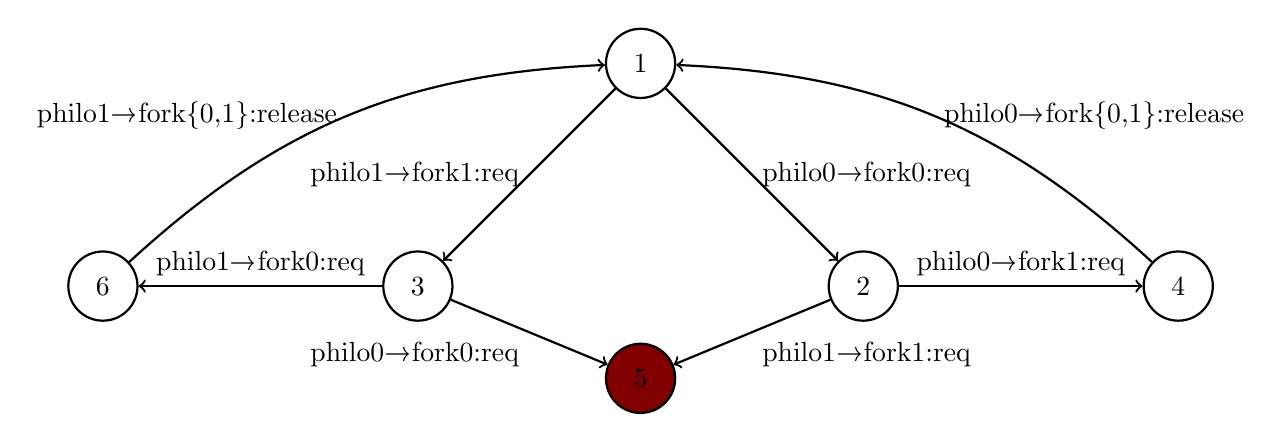
\begin{tikzpicture}[node distance={40mm}, thick, main/.style = {draw, circle}] 
        \node[state] (n_1) {1};
        \node[state] (n_2) [below right of=n_1] {2};
        \node[state] (n_3) [below left of=n_1] {3};
        \node[state] (n_4) [right of=n_2] {4};
        \node[state] (n_5) [below of=n_1, fill=red] {5};
        \node[state] (n_6) [left of=n_3] {6};
        
        \draw[->] (n_1) -- node[midway, right, pos=0.5] {philo0→fork0:req} (n_2);
        \draw[->] (n_1) -- node[midway, left, pos=0.5] {philo1→fork1:req} (n_3);
        \draw[->] (n_2) -- node[midway, below right, pos=0.5] {philo1→fork1:req} (n_5);
        \draw[->] (n_3) -- node[midway, below left, pos=0.5] {philo0→fork0:req} (n_5);
        \draw[->] (n_2) -- node[midway, above, pos=0.5] {philo0→fork1:req} (n_4);
        \draw[->] (n_4) to[bend right=20] node[midway, right, pos=0.5] {philo0→fork\{0,1\}:release} (n_1);
        \draw[->] (n_3) -- node[midway, above, pos=0.5] {philo1→fork0:req} (n_6);
        \draw[->] (n_6) to[bend left=20] node[midway, left, pos=0.5] {philo1→fork\{0,1\}:release} (n_1);
      \end{tikzpicture}
    }
  % }%
  \caption{Global view of the dining philosophers example.}
  \label{graph:philosophers}
\end{figure}
\subsection{Bank account}
This case study is taken from the \texttt{account} example from the benchmark 
suite of the tool.
We now consider a system where a bank account is accessed
by two clients, dubbed C1 and C2.
% 
\tikzset{
	hpath/.style={
			very thick,
			line cap = round,
			line join = round,
			line width=0.1cm,
			opacity=.70,
			color = teal!30
		}
}

\begin{lstlisting}
account(Value) ->
  receive
    read from Client ->
      send Value to Client,
      account(Value);
    NewValue from Client ->
      account(NewValue).

client() ->
  send read to Acc,
  receive Value from Acc,
  % operations on Value
  send NewValue to Acc.
\end{lstlisting}

The pseudocode yields the behavior of the bank account,
where $\mathsf{Value}$ represents its current balance.
This process waits for requests from a client.
A request can either be a \lstinline{read} access to know
the current balance or an update request of such value to a
\lstinline{NewValue}.

Symmetrically, client processes C1 and C2 behave according to the
pseudocode on the left: the process reads the current balance
from the account,
performs some internal operations based on such value, and
updates the balance.
%
The global view of the communicating system is depicted in
Figure~\ref{fig:account}.

\newcommand\dummy{C}
\begin{figure}[!ht]
	\centering
	\begin{tikzpicture}[node distance={27mm}, scale = .6, transform shape, thick, main/.style = {draw, circle}]
		\node (n_1) [state] {};
		\node (n_2) [state, below left of=n_1] {};
		\node (n_3) [state, below right of=n_1] {};
		\node (n_4) [state, left= 3.5cm of n_2] {4};
		\node (n_5) [state, below=3cm of n_1] {};
		\node (n_6) [state, right= 3.5cm of n_3] {6};
		\node (n_7) [state, below of=n_4] {7};
		\node (n_8) [state, below left of=n_5] {};
		\node (n_9) [state, below right of=n_5] {};
		\node (n_10) [state, below of=n_6] {10};
		\node (n_11) [state, accepting, below= of n_7] {11};
		\node (n_12) [state, accepting, below=1.5cm of n_8] {};
		\node (n_13) [state, accepting, below= 1.5cm of n_9] {};
		\node (n_14) [state, accepting, below=2.5cm of n_10] {14};

		\draw[->] (n_1) -- node[midway, above left] {acc→\dummy1:Value} (n_2);
		\draw[->] (n_2) -- node[midway, below left] {acc→\dummy2:Value} (n_5);
		\draw[->] (n_5) -- node[midway, above left=-2mm] {\dummy1→acc:NewValue} (n_8);
		\draw[->] (n_8) -- node[midway, below left] {\dummy2→acc:NewValue} (n_12);

		\draw[->] (n_1) -- node[midway, above right] {acc→\dummy2:Value} (n_3);
		\draw[->] (n_3) -- node[midway, below right] {acc→\dummy1:Value} (n_5);
		\draw[->] (n_5) -- node[midway, above right=-2mm] {\dummy2→acc:NewValue} (n_9);
		\draw[->] (n_9) -- node[midway, below right] {\dummy1→acc:NewValue} (n_13);

		\draw[hpath] ($(n_1.center) + (-5pt,-5pt)$) -- (n_2.center) -- (n_5.north west) -- ($(n_5.center)+(-5pt,0)$) -- (n_5.south west) -- (n_8.center) -- ($(n_12.center) + (0pt,5pt)$);
		\draw[hpath] ($(n_1.center) + (5pt,-5pt)$) -- (n_3.center) -- (n_5.north east)  -- ($(n_5.center)+(5pt,0)$) -- (n_5.south east)  -- (n_9.center) -- ($(n_13.center) + (0pt,5pt)$);

		\foreach \n in {1,2,3,5,8,9,12,13}{
				\node at (n_\n) {\n};
			}

		\draw[->] (n_2) -- node[midway, above=3mm] {C1→acc:NewValue} (n_4);
		\draw[->] (n_4) -- node[midway, above left] {acc→C2:Value} (n_7);
		\draw[->] (n_7) -- node[midway, above left] {C2→acc:NewValue} (n_11);

		\draw[->] (n_3) -- node[midway, above=3mm] {C2→acc:NewValue} (n_6);
		\draw[->] (n_6) -- node[midway, above right] {acc→C1:Value} (n_10);
		\draw[->] (n_10) -- node[midway, above right] {C1→acc:NewValue} (n_14);
	\end{tikzpicture}
	\caption{Global view of the bank account example}
	\label{fig:account}
\end{figure}

We can observe two correct executions where the operations are
performed in a read-update-read-update order (taking the path via
states 1-2-4-7-11 or the one via states 1-3-6-10-14).
%
However, there is also a read-read-update-update order on the
highlighted paths.
%
Although the choreography is not inherently incorrect, these
highlighted paths could represent a violation of mutual exclusion
which may be undesirable for developers in certain
contexts.
The choreography automaton in Figure~\ref{fig:account} helps in spotting
this issue.

%%% Local Variables:
%%% mode: LaTeX
%%% TeX-master: "main"
%%% End:


\section{Conclusion}
The project began with the goal of creating a proof of concept, a prototype,  
for an analyzer that could extract choreography automata directly
from an existing codebase, which is quite unique in its field,
having a bottom-up over-approximation approach leaning to mainstream
programming languages.  
A significant amount of effort and resources have been invested,  
primarily in the tool's codebase and its design around examples and  
use cases. Additionally, extensive discussions have taken place  
regarding the high-level and general aspects of the tool.  

The results of this prototype are promising, demonstrating that such  
a tool is feasible and worth further exploration.  
We discussed on how the analysis should work, defining motivations,  
requirements, and challenges surrounding the tool. At the same time,  
we have introduced multiple improvements to the existing codebase to  
refine its output.  

Finally, efforts have been made to advance a formalization process,  
highlighting what has been done well and what still needs  
improvement. This has provided valuable insights into the tool’s  
design and future directions.  

The formalization process has just begun and will require further refinement  
in the future. A new testing method for the tool has been introduced, but  
additional effort is needed to generate correct global views. This is  
crucial for properly assessing the tool's precision and could lead to  
refinements in its existing components.  

The formalization process has also highlighted the need to refactor the  
local view component. A possible improvement is the addition of a parsing  
module capable of reading local views from files (e.g., DOT format).  
This enhancement would make the tool more general, removing its strict  
dependency on Erlang programs. 
With such a feature, developers could create a separate tool to translate  
their preferred programming language into a local view, outputting it  
as a DOT file. This file could then be provided as input to our tool  
to compute the corresponding global specification, making it a more  
versatile and widely applicable solution.  

Another area for improvement is the minimization and post-processing  
module. It can be expanded with better heuristics to generate clearer,  
more structured, and easily interpretable graphs. Enhancing these  
optimizations will improve readability and usability, making the tool’s  
output more insightful and practical.


\subsection{Related works}
In the industrial context, Erlang's actor model has also inspired other 
programming languages or frameworks, such as Elixir \cite{website:elixir}, a 
programming language based on Erlang's virtual machine. Other programming 
languages also implement the actor model, such as Go \cite{website:golang} with 
its GoRoutines (comparable to Erlang's spawns) and channels (similar to Erlang's
send and receive).
Software industry is increasingly devoting attention to choreographic approaches
\cite{BPMN,bon18,fmmt20,DBLP:journals/software/AutiliIT15} because
they naturally support modularization and decoupling.
%
In fact, distributed components coordinate according to a global
description without the need of an explicit coordinator.
%
In the academic context, research in the field of \textit{choreography} focuses 
on two main topics: \textit{choreography specification} and 
\textit{choreographic programming}.
\begin{itemize}
    \item \textit{Choreography specifications}: this area includes formal 
    methods, such as multiparty asynchronous session types 
    \cite{honda2008multiparty}, which have been established to describe the 
    interactive structure of a fixed number of actors from a global perspective.
    These methods enable the syntactic verification of actors' correctness by 
    projecting the global specification onto individual participants. 
    Choreography specifications are also studied as contracts, which provide 
    abstract descriptions of program behavior, known as \textit{multiparty 
    contracts} \cite{zava}.
    \item \textit{Choreographic programming}: this programming paradigm has been
    explored both theoretically, as in \cite{website:wscdl}, and industrially, 
    as in \cite{website:bpmn}. Several choreographic programming languages have
    been designed and studied to support this paradigm \cite{montesi2010jolie, 
    montesi2014choreographic, giallorenzo2020object, dalla2014aiocj}.
\end{itemize}
In this context, global specifications are crucial for guaranteeing
correctness (since they are blueprints of complex distributed systems
and feature model-driven development) as well as for program
comprehension. 
Most formal works on communication protocol 
specifications emphasize the projection of a global specification onto local 
specifications. However, the process of choreography extraction remains 
challenging and has been explored in \cite{cflm17}, with a general 
framework for extracting choreographies presented in 
\cite{cruz2022implementing}.
%
To the best of our knowledge, the first attempts to extract global
specifications for message-passing systems goes back
to~\cite{myh09,lt12,lty15}.
%
These approaches aim to identify ``meaningful" global specifications
according to general properties such as deadlock-freedom or absence of
orphan messages~\cite{bz83}.
%
A limitation of these approaches is that they do not start from
components written in a full-fledged programming language.
%
Rather, distributed components are specified in~\cite{lt12,lty15} as
abstract models (respectively, $\pi$-calculus
processes~\cite{sw02,mil99,mpw92} and communicating finite-state
machines~\cite{bz83}).


%%% Local Variables:
%%% mode: LaTeX
%%% TeX-master: "main"
%%% End:

\subsection{State of the Art}
\label{sota}
\todo{già messo nel DoW, ci sta ripeterlo? io forse lo toglierei}
In the industrial context, Erlang's actor model has also inspired other 
programming languages or frameworks, such as Elixir \cite{website:elixir}, a 
programming language based on Erlang's virtual machine. Other programming 
languages also implement the actor model, such as Go \cite{website:golang} with 
its GoRoutines (comparable to Erlang's spawns) and channels (similar to Erlang's
send and receive).

\bigskip

In the academic context, research in the field of \textit{choreography} focuses 
on two main topics: \textit{choreography specification} and 
\textit{choreographic programming}.
\begin{itemize}
    \item \textit{Choreography specifications}: this area includes formal 
    methods, such as multiparty asynchronous session types 
    \cite{honda2008multiparty}, which have been established to describe the 
    interactive structure of a fixed number of actors from a global perspective.
    These methods enable the syntactic verification of actors' correctness by 
    projecting the global specification onto individual participants. 
    Choreography specifications are also studied as contracts, which provide 
    abstract descriptions of program behavior, known as \textit{multiparty 
    contracts} \cite{zava}.
    \item \textit{Choreographic programming}: this programming paradigm has been
    explored both theoretically, as in \cite{website:wscdl}, and industrially, 
    as in \cite{website:bpmn}. Several choreographic programming languages have
    been designed and studied to support this paradigm \cite{montesi2010jolie, 
    montesi2014choreographic, giallorenzo2020object, dalla2014aiocj}.
\end{itemize}

A way to formalize choreographies is through Choreographic Automata 
\cite{barbanerachoreography}, which describe a communication system using a 
finite-state automaton. By using this model, it is possible to use the results 
of automaton studies to demonstrate the mentioned properties 
\cite{orlando2021corinne}. Most formal works on communication protocol 
specifications emphasize the projection of a global specification onto local 
specifications. However, the process of choreography extraction remains 
challenging and has been explored in \cite{cruz2017paths}, with a general 
framework for extracting choreographies presented in 
\cite{cruz2022implementing}. In our work, we aim at extracting choreographies 
from an existing and widely-used programming language like Erlang, despite it 
not being originally designed with choreography in mind.

\newpage

\bibliographystyle{plain}
\bibliography{ref}

\end{document}
